\atstartofhistorysection
\section[Un peu d’histoire : le nombre de temps moteur]{Un peu d’histoire :\onlyamphibook{\\} le nombre de temps moteur}
\label{ch_deux_temps}

	Historiquement, nous avons appris à transformer de la chaleur en travail en manipulant des quantités fixes de fluide emprisonné dans des enclaves. Ces enclaves ont toujours été de géométrie cylindrique, ce qui facilite grandement la fabrication des pistons qui exploitent les variations de volume du fluide pour en extraire du travail.
	
	Lorsque le fluide est de l’eau, l’apport de chaleur se fait dans une chaudière et la vapeur est \emph{ensuite} transférée dans le ou les cylindres pour y être détendue (\S\ref{ch_cycles_moteurs_vapeur}). À la fin du \textsc{xix}\ieme siècle toutefois, on commence à utiliser de l’air, un fluide à l’intérieur duquel on peut directement créer la chaleur par combustion. Le processus complexe consistant jusqu’alors à effectuer une combustion séparée pour chauffer une chaudière métallique qui elle-même chauffe enfin l’eau du moteur est éliminé avec toutes les pertes de chaleur et de température qu’il engendre. C’est la naissance du moteur \vocab{à combustion interne}, dont le développement sera notamment porté par les ingénieurs allemands \wf{Nikolaus Otto} et \wf{Rudolf Diesel} (\S\ref{ch_moteurs_alternatifs}). On réalise désormais la combustion et la détente au même endroit, directement dans le cylindre.
	
	Cependant, pour effectuer une combustion interne, il faut résoudre un nouveau problème : comme l’oxygène de l’air est utilisé pendant la combustion, celle-ci ne peut être effectuée qu’une seule fois. Après chaque combustion, il est donc indispensable de rejeter hors du cylindre les produits de réaction ($\text{CO}_2$ et $\text{H}_2\text{O}$ essentiellement) et d’y ré-insérer de l’air «~frais~» contenant l’oxygène $\text{O}_2$ nécessaire à la rupture des molécules d’hydrocarbures $\text{C}_x\text{H}_y$ produisant la chaleur. Deux solutions différentes sont alors adoptées.
	
	La méthode la plus courante est de consacrer un mouvement de piston à chaque étape : le premier pour la compression, le second pour la détente (après ou pendant la combustion), le troisième pour rejeter les gaz brûlés (échappement), et le dernier pour admettre de l’air frais (aspiration). Les moteurs suivant ce procédé sont dits \vocab{à quatre temps} (\cref{fig_quatre_temps}), et ils ont toujours été les plus utilisés.
	
	\onlyamphibook{\begin{figure}[htb!]}%handmade
	\onlyframabook{\begin{figure}}
		\begin{center}
			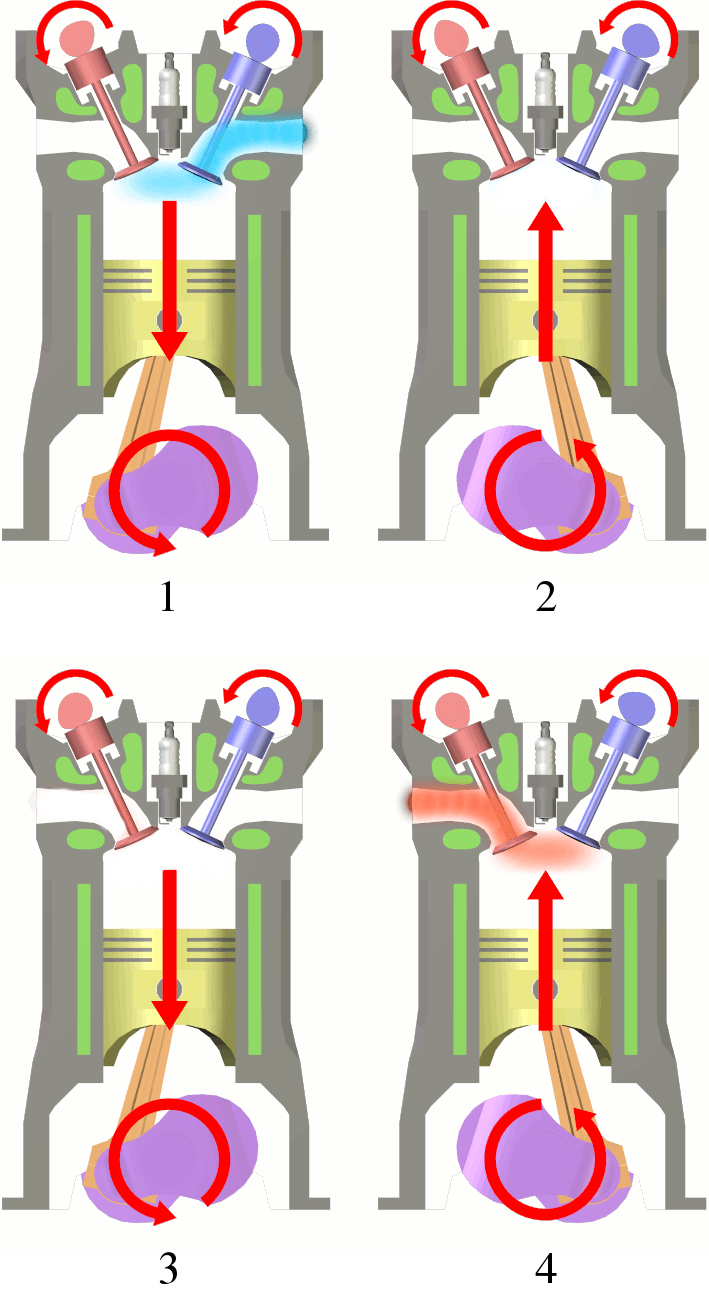
\includegraphics[width=6cm]{images/four_stroke_cycle.png}
			\supercaption{Les quatre étapes d’un moteur à quatre temps. Le piston descend pour admettre de l’air frais arrivant de la droite (\vocab{admission}, 1) ; il monte ensuite pour augmenter la température de l’air (\vocab{compression}, 2) ; la production de travail utile a lieu pendant une descente (\vocab{détente}, 3) ; enfin l’air est rejeté à l’extérieur lors d’un quatrième et dernier mouvement (\vocab{échappement}), 4) avant de recommencer le cycle. La plupart des moteurs à pistons-cylindres actuels suivent ce procédé.}%
			{schémas \wcfile{Four stroke cycle intake.png}{1} \wcfile{Four stroke cycle compression.png}{2} \wcfile{Four stroke cycle power.png}{3} \wcfile{Four stroke cycle exhaust.png}{4} \ccby par \weun{Wapcaplet}{Eric Pierce}}
			\label{fig_quatre_temps}
		\end{center}
	\end{figure}
	
	La seconde méthode ne manquera pas de surprendre les puristes : il s’agit d’effectuer ces quatre opérations en \vocab{deux temps} seulement. Dans ces moteurs, une partie de l’expansion des gaz est consacrée à leur échappement, qui est effectué simultanément à l’admission d’air (figures~\ref{fig_cycle_deux_temps} et~\ref{fig_pv_deux_temps}). Assurément, aucune des quatre étapes ne peut être effectuée de façon optimale : les phases de compression et détente ne sont effectuées que sur une partie du débattement, et la vidange est nécessairement incomplète à cause du mélange des gaz frais et usagés. Par contre, les combustions sont deux fois plus fréquentes, puisqu’on se dispense des temps d’admission et d’échappement pendant lesquels aucune opération thermodynamique n’a lieu. Ainsi, à cylindrée et vitesse de rotation égales, les moteurs à deux temps sont beaucoup plus puissants que leurs homologues à quatre temps, même s’ils sont aussi nettement moins efficaces.
	
	\begin{figure}
		\begin{center}
			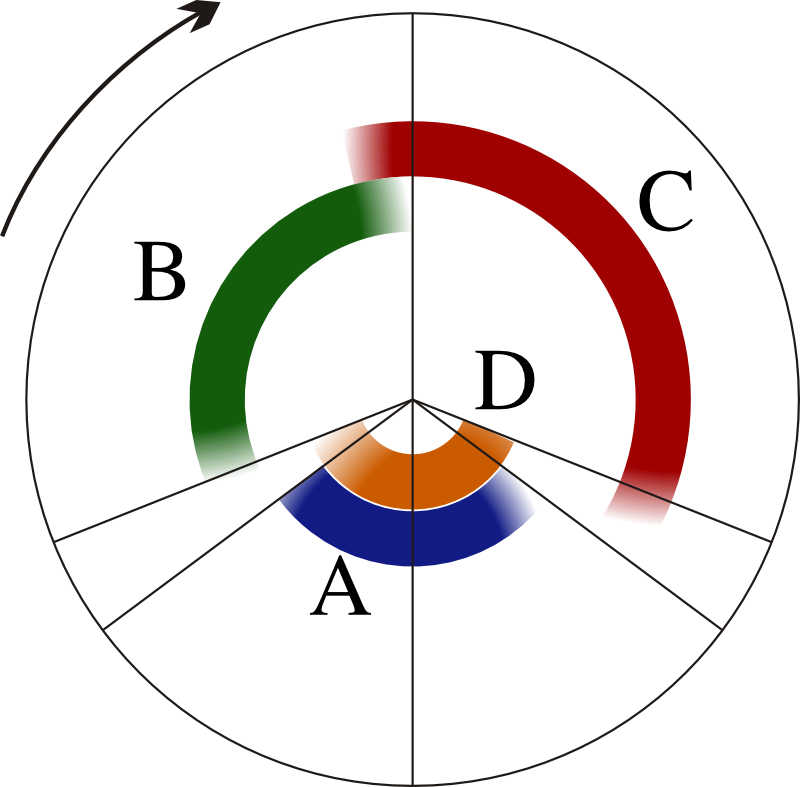
\includegraphics[width=6cm]{images/cycle_deux_temps.png}
			\supercaption{Cycle d’un moteur deux-temps. Les quatre étapes nécessaires au fonctionnement sont effectuées sur une seule révolution de vilebrequin, soit deux mouvements de piston. L’admission (A) se fait pendant le passage au point mort bas, la compression (B) débute tard et la détente (C) est interrompue pour permettre la vidange (D) lorsque le piston se rapproche à nouveau du point mort bas.}%
			{schéma dérivé d’\wcfile{Ciclo del motore 2T unidirezionale.svg}{un schéma} \ccbysa par \wcu{A7N8X}}
			\label{fig_cycle_deux_temps}
		\end{center}
	\end{figure}	
	
	\begin{figure}
		\begin{center}
			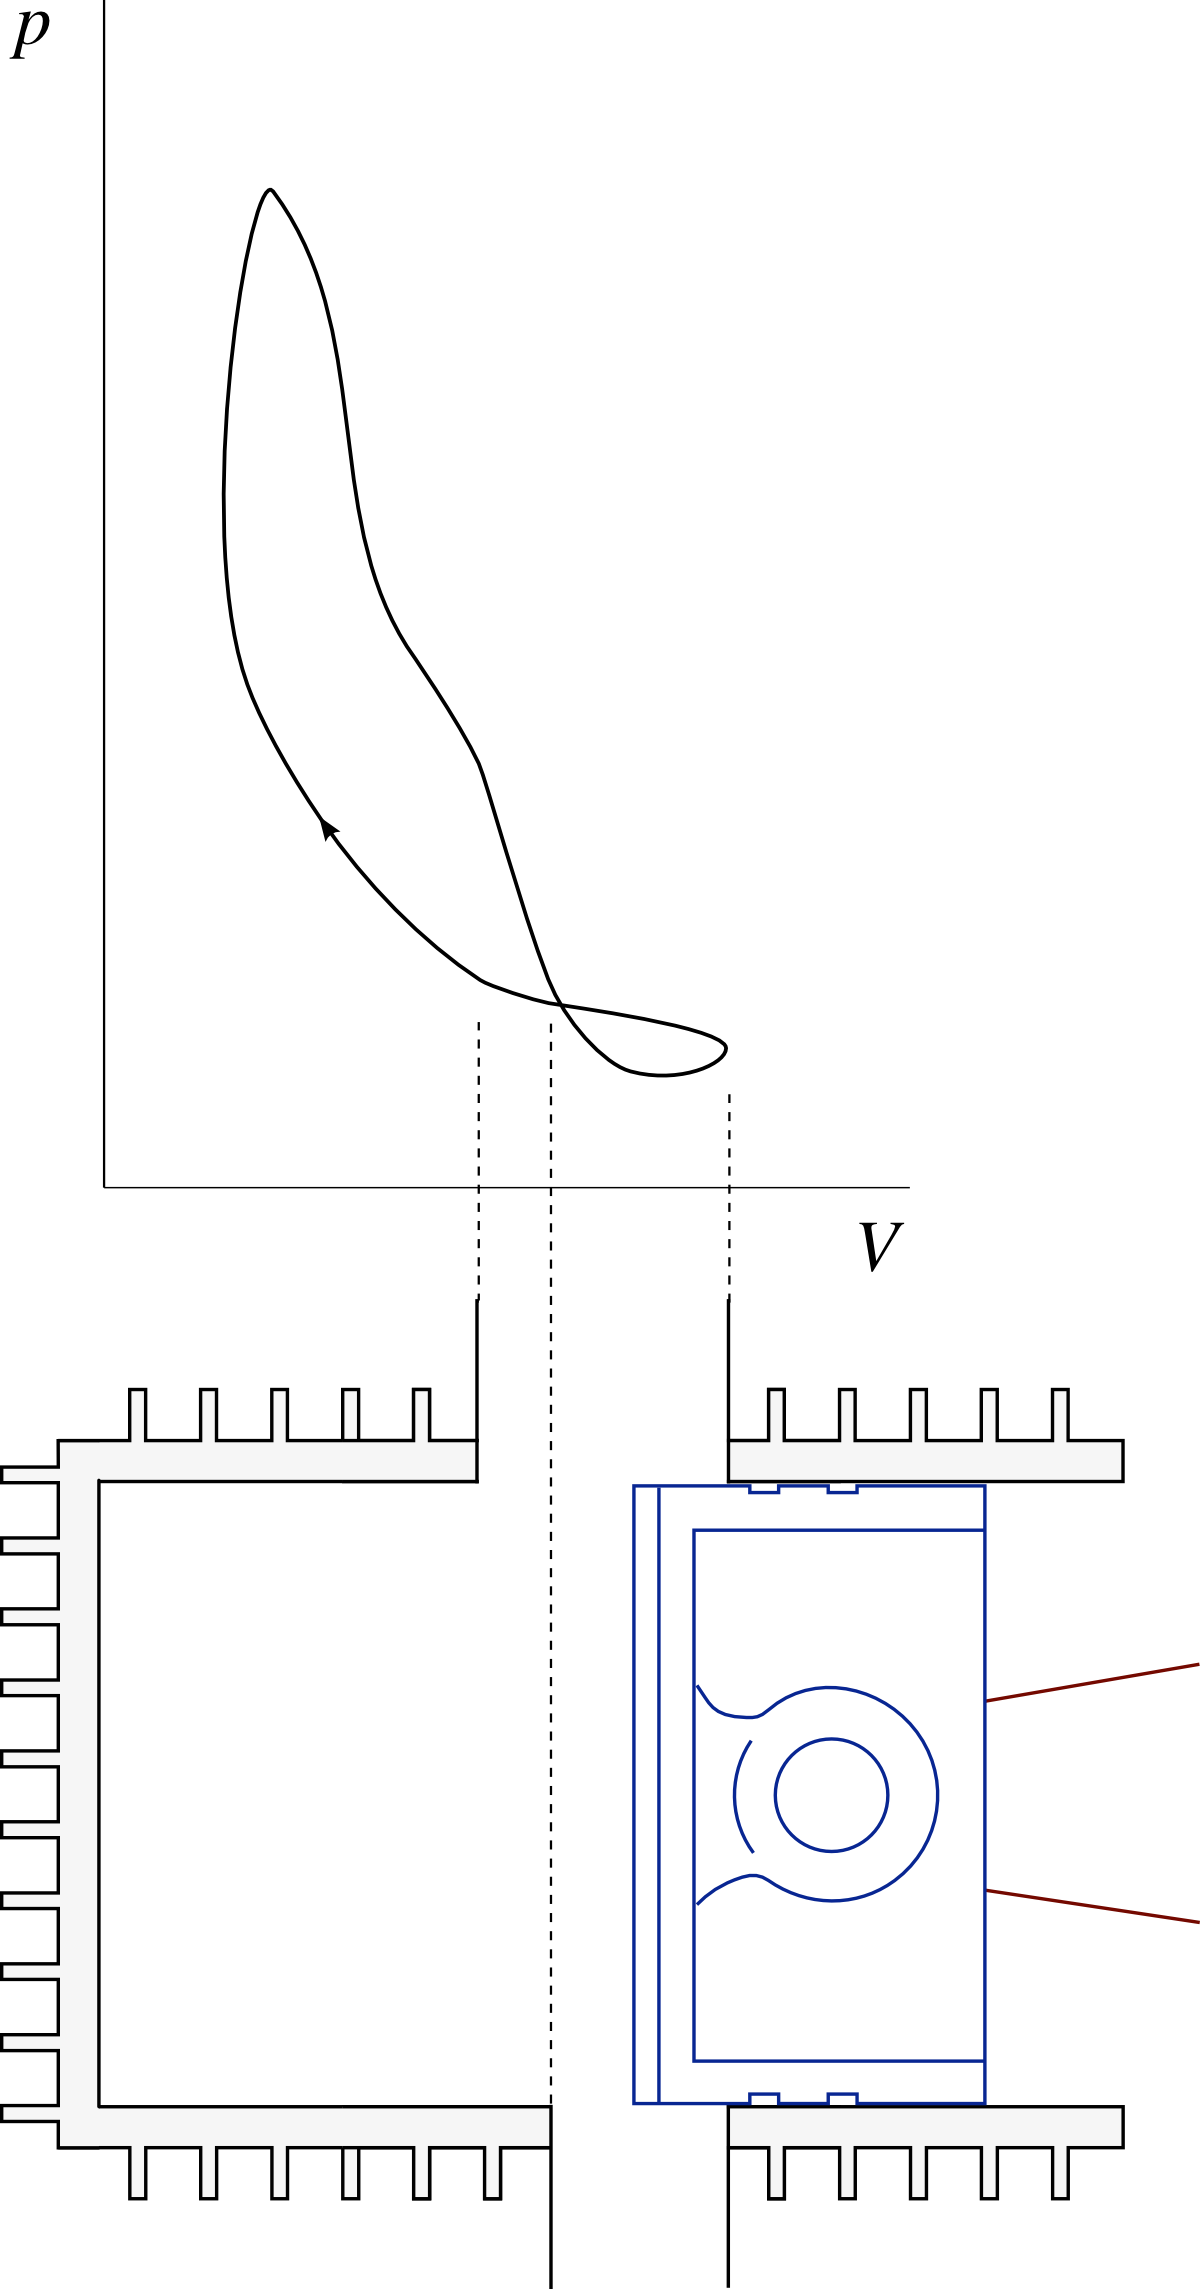
\includegraphics[width=6cm]{images/pv_deux_temps.png}
			\supercaption{Diagramme pression-volume schématique du cylindre d’un moteur deux-temps à admission carter. Il est laissé à l’étudiant/e le loisir de retrouver laquelle des deux lumières (haute ou basse) correspond à l’admission et à l’échappement dans le cylindre.}%
			{schéma dérivé d’\wcfile{Motor 2 timpi.png}{un schéma} \ccbysa par \wcu{Terraflorin}}
			\label{fig_pv_deux_temps}
		\end{center}
	\end{figure}
	
	Le développement du moteur à deux temps est conjoint à celui du moteur quatre-temps, mais son développement connaîtra son plus grand essor après la seconde guerre mondiale. Le perfectionnement par l’ingénieur allemand \we{Walter Kaaden} d’un ingénieux système d’échappement, dont la seule géométrie augmente le débit d’air s’échappant pendant les détentes et le réduit lors des compressions, rend alors le moteur très compétitif sur les motos de course ; ce \vocab{pot de détente accordé} (\cref{fig_pot_detente_accorde}) sera adopté sur de nombreux modèles de production. 	
	
	\begin{figure}
		\begin{center}
			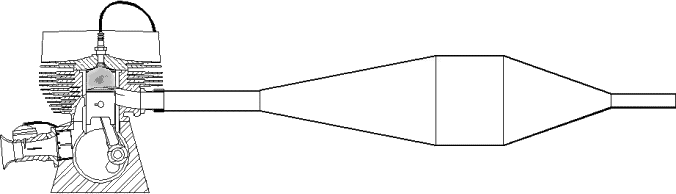
\includegraphics[width=\textwidth]{images/pot_detente_accorde.png}
			\supercaption{Pot de détente accordé (parfois dit "harmonique") monté sur un moteur deux-temps. Comme l’écoulement est instationnaire, il est possible de jouer sur la pression qu’exercent les quantités fixes de gaz rejetés sur la lumière d’échappement lorsqu’ils traversent le pot. La traversée de la partie expansive réduit la pression (et facilite donc la vidange pendant la descente du piston), tandis que le passage dans le rétrécissement, au contraire, augmente cette pression (et réduit donc les pertes de gaz pendant la remontée du piston).}%
			{\wcfile{Arbeitsweise Zweitakt.gif}{schéma} \ccbysa par Achim Agster}
			\label{fig_pot_detente_accorde}
		\end{center}
	\end{figure}
	
	En parallèle, les idées formulées par l’entrepreneur anglais \we{Joseph Day} à la fin du \textsc{xix}\ieme siècle sur le mécanisme contrôlant l’admission se diffusent très largement. Avec son astucieuse \vocab{admission par carter}, c’est le piston lui-même qui sert de valve (\cref{fig_admission_carter}). L’air d’admission passe tout d’abord par le carter où tourne le vilebrequin, puis il est légèrement comprimé par le mouvement du piston pendant la détente avant de pouvoir entrer dans le cylindre. Le moteur fonctionne ainsi sans aucune soupape mobile ; la lubrification peut même être assurée simplement par injection d’huile directement dans l’air d’admission.
	
	\begin{figure}
		\begin{center}
			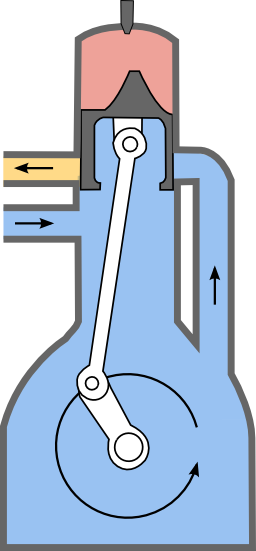
\includegraphics[width=4cm]{images/admission_carter.png}
			\supercaption{Système d’admission par carter. L’air d’admission, chargé de carburant destiné à la combustion et d’huile destinée à lubrifier les pièces mécaniques, pénètre d’abord dans le carter du vilebrequin. Il est comprimé puis inséré dans le cylindre avec le seul mouvement descendant du piston. Il n’y a besoin d’aucune valve ou soupape.}%
			{\wcfile{Silnik dwusuwowy.svg}{schéma} \pd par \wcu{Tomeq183}}
			\label{fig_admission_carter}
		\end{center}
	\end{figure}

	Avec ces deux atouts, le moteur trouve son application partout où les contraintes de poids, de volume, de coût d’acquisition et de maintenance priment sur l’efficacité. Après avoir propulsé trois millions de \textit{Trabant} en Allemagne de l’Est, il a été adopté sur la quasi-totalité des outils portatifs extérieurs (tronçonneuses, tondeuses, etc.). Le moteur se miniaturise sans difficulté, laisse de la place pour les jambes à bord d’un scooter, permet aux motoneiges de démarrer facilement, bref, jusqu’aux années 90 rien --pas même les associations de voisinage !-- ne semblait pouvoir freiner sa progression.

	Au début du \textsc{xxi}\ieme siècle, il faut pourtant renoncer à ces attraits. On peut de guerre lasse accepter le son irritant dégagé par le moteur à deux temps, mais ses émissions polluantes sont effarantes. La lubrification par injection d’huile dans l’air d’admission provoque le rejet atmosphérique de fumées, odeurs et particules nocives. En outre, la vidange toujours très incomplète du cylindre limite fortement l’efficacité de la combustion et le rendement thermique. Le durcissement des réglementations contrôlant les émissions force ainsi progressivement le remplacement de ces moteurs par d’autres à quatre temps ou par des systèmes électriques -- dont les batteries sont bien souvent chargées avec de l’énergie provenant de centrales électriques… à vapeur. On voit que des décisions technologiques a priori mineures ont parfois des conséquences à l’échelle planétaire !
	
\atendofhistorysection
